\documentclass[12pt,a4paper]{article}

% ── Packages ──────────────────────────────────────────────────────────────────
\usepackage[margin=1in]{geometry}
\usepackage{amsmath}
\usepackage{graphicx}
\usepackage{booktabs}
\usepackage{array}
\usepackage{hyperref}
\usepackage{setspace}
\usepackage{titlesec}
\usepackage{parskip}
\usepackage{enumitem}
\usepackage{fancyhdr}
\usepackage{xcolor}
\usepackage{tikz}
\usetikzlibrary{shapes.geometric, arrows.meta, positioning, calc}
\usepackage{caption}
\usepackage{listings}
\usepackage{tabularx}
\usepackage{multirow}
\usepackage{tcolorbox}
\usepackage{mdframed}
\usepackage{float}
\usepackage{booktabs}

% ── Hyperref setup ────────────────────────────────────────────────────────────
\hypersetup{colorlinks=true, linkcolor=blue!60!black,
            urlcolor=blue!60!black, citecolor=blue!60!black}

% ── Code listing style ────────────────────────────────────────────────────────
\lstset{basicstyle=\ttfamily\small, breaklines=true, frame=single,
        backgroundcolor=\color{gray!8}, numbers=left,
        numberstyle=\tiny\color{gray}, numbersep=5pt, xleftmargin=10pt}

% ── Colour definitions ────────────────────────────────────────────────────────
\definecolor{svblue}{RGB}{31, 111, 235}
\definecolor{svgreen}{RGB}{63, 185, 80}
\definecolor{svamber}{RGB}{210, 153, 34}
\definecolor{svred}{RGB}{248, 81, 73}

% ── Header / Footer ───────────────────────────────────────────────────────────
\pagestyle{fancy}
\fancyhf{}
\lhead{\small MIT Manipal \quad SecViz --- MADLAB Partial Report}
\rfoot{\thepage}
\renewcommand{\headrulewidth}{0.4pt}

% ── Section formatting ────────────────────────────────────────────────────────
\titleformat{\section}{\large\bfseries\color{svblue}}{\thesection}{1em}{}[\titlerule]
\titleformat{\subsection}{\normalsize\bfseries}{\thesubsection}{1em}{}

% ── Convenience commands ──────────────────────────────────────────────────────
\newcommand{\SV}{\textit{SecViz}}
\newcommand{\tick}{\textcolor{svgreen}{$\checkmark$}}
\newcommand{\cross}{\textcolor{svred}{$\times$}}

\newmdenv[backgroundcolor=svblue!5, linecolor=svblue!40, linewidth=1pt,
          roundcorner=4pt, innerleftmargin=10pt, innerrightmargin=10pt,
          innertopmargin=6pt, innerbottommargin=6pt]{infobox}

% ══════════════════════════════════════════════════════════════════════════════
\begin{document}

% ── Title page ────────────────────────────────────────────────────────────────
\begin{titlepage}
    \centering
    \vspace*{1.5cm}
    {\large\bfseries MANIPAL INSTITUTE OF TECHNOLOGY\\
    \normalsize A Constituent Unit of MAHE, Manipal\par}
    \vspace{0.6cm}
    \rule{\linewidth}{1.5pt}\par
    \vspace{0.4cm}
    {\small MADLAB Project Partial Report\par}
    \vspace{0.3cm}
    {\Huge\bfseries\color{svblue} SecViz\par}
    \vspace{0.2cm}
    {\LARGE\bfseries An Interactive Android Application for\\[4pt]
    Binary Exploitation Education\par}
    \vspace{0.4cm}
    \rule{\linewidth}{1.5pt}\par
    \vspace{1.2cm}

    {\normalsize\bfseries Team Members:\par}
    \vspace{0.4cm}
    \begin{tabular}{ll}
        Mrityunjai Bhatt    & 230953302 \\[4pt]
        Noorain Eqbal       & 230953454 \\[4pt]
        Parth Verma         & 230953436 \\[4pt]
        Shashank Chaudhary  & 230953402
    \end{tabular}

    \vspace{1.2cm}
    {\normalsize\bfseries Under the Guidance of\par}
    \vspace{0.3cm}
    \begin{tabular}{cc}
        \multicolumn{2}{c}{[Guide Name]} \\
        \multicolumn{2}{c}{School of Computer Engineering} \\
        \multicolumn{2}{c}{Manipal Institute of Technology, MAHE, Manipal}
    \end{tabular}

    \vfill
    {\normalsize School of Computer Engineering\\
    Manipal Institute of Technology, MAHE, Manipal\par}
    \vspace{0.4cm}
    {\normalsize April 2026\par}
\end{titlepage}

\tableofcontents
\newpage

% ══════════════════════════════════════════════════════════════════════════════
\section{Abstract}

\SV{} is a native Android application for interactive, animated education in
binary exploitation and low-level computer security. Most existing resources in
this space are either text-heavy or require deep familiarity with command-line
debuggers, creating a significant barrier for students new to the domain.
\SV{} removes this barrier by simulating real exploitation techniques---buffer
overflows, information leaks, control-flow hijacking, and Return-Oriented
Programming---directly on a mobile device with step-by-step animated state
transitions and no prerequisite toolchain.

The application is structured as a progressive level system. Level~1 demonstrates
a stack buffer overflow causing a segmentation fault; Level~2A visualises a
null-terminator memory leak; Level~2B simulates control-flow hijacking to a
\texttt{win()} function, featuring an in-app \texttt{objdump} viewer and a
three-step interactive payload builder wizard. Upcoming levels cover ROP gadget
chaining and security mitigations (stack canary, PIE/ASLR).

Built natively for Android (API~26+) in Java following the MVVM pattern, \SV{}
renders its stack as a live, animated custom \texttt{StackCanvasView}, supports
register-state time-travel debugging, and includes a hex dump drawer and snapshot
timeline.

% ══════════════════════════════════════════════════════════════════════════════
\section{Introduction}

Understanding binary exploitation requires simultaneously reasoning about C source
code, compiled machine instructions, live register state, and stack frame structure.
Existing teaching resources---textbooks~\cite{erickson2008}, CTF
competitions~\cite{chapmanburket2016}, and debugger-guided walkthroughs---each
serve a role, but all assume toolchain familiarity that acts as a barrier for
students new to the domain.

Research in computing education provides a clear direction. Guo~\cite{guo2013}
showed that step-by-step stack frame visualisations significantly improve
conceptual understanding among novice programmers. Hundhausen et al.\
\cite{hundhausen2002} established that active interaction with a visualisation
system substantially outperforms passive observation of static diagrams.
Both findings converge on the same conclusion: the medium matters as much as
the content.

\SV{} is built on this evidence. It delivers the binary exploitation curriculum
inside an animating, interactive Android interface with no prerequisite tooling.
A learner can step through a \texttt{gets()} call, watch the stack fill and
overflow in real time, open the in-app \texttt{objdump} to locate \texttt{win()},
construct a payload with the tap-based wizard, press ``Exploit'', and observe the
animated control-flow redirect---all on a smartphone.

\begin{infobox}
\textbf{Design Principle:}\quad Every concept a learner of binary exploitation must
understand---stack layout, buffer boundaries, return address position, register state,
assembly mnemonics---is made simultaneously visible, interactive, and animated on the
same screen at the moment it becomes relevant to the execution trace.
\end{infobox}

% ══════════════════════════════════════════════════════════════════════════════
\section{Literature Survey}

\paragraph{Program Execution Visualisation.}
Guo~\cite{guo2013} developed Python Tutor and found that step-by-step rendering of
stack frames significantly improved comprehension among novice learners. \SV{}'s
\texttt{StackCanvasView} operationalises this finding in the security domain: each
\texttt{handleNextStep()} call advances the execution trace and re-renders the
stack live.

\paragraph{Interactive Visualisation in CS Education.}
Hundhausen et al.~\cite{hundhausen2002} found that learners who actively engaged
with a visualisation system substantially outperformed those observing static
diagrams. This motivates \SV{}'s design of requiring the learner to take active
steps: selecting junk fill ranges, tapping stack blocks, entering hex addresses,
and pressing ``Exploit'' rather than reading pre-drawn attack diagrams.

\paragraph{CTF-Based Cybersecurity Education.}
Chapman and Burket~\cite{chapmanburket2016} evaluated CTF competitions as a
pedagogical tool, reporting skill improvement but identifying a critical limitation:
CTF platforms assume prior debugger familiarity and offer no guided visual
explanation of internal memory changes. \SV{} provides exactly the guided,
step-by-step animated explanation that CTF platforms omit.

\paragraph{Cryptographic Education.}
Rescorla~\cite{rescorla2018} demonstrated that concrete analogies (colour mixing
for Diffie--Hellman) improve conceptual clarity for learners without modular
arithmetic backgrounds. \SV{}'s planned cipher modules extend this principle to
interactive mobile touchscreen manipulation.

\paragraph{Stack Buffer Overflow.}
Erickson~\cite{erickson2008} provided the foundational treatment of stack-based
buffer overflow via debugger-based experiments. \SV{} Levels~1 and~2B
operationalise the same content in an animated, zero-toolchain mobile format.

\paragraph{Return-Oriented Programming.}
Shacham~\cite{shacham2007} introduced gadget chaining to bypass NX/DEP
protections. Understanding ROP demands simultaneous reasoning about binary layout
and stack state across multiple function boundaries---a cognitive load \SV{}'s
Level~3 addresses through a symbolic gadget chain editor with live hex-byte
resolution.

% ── 3.1 Comparison Table ─────────────────────────────────────────────────────
\subsection{Comparison of Related Work}

\begin{table}[H]
\centering
\caption{Related work vs \SV{} feature profile}
\label{tab:comparison}
\renewcommand{\arraystretch}{1.3}
\begin{tabular}{>{\bfseries}p{3.4cm} p{3cm}
                >{\centering}p{1.5cm} >{\centering}p{1.5cm}
                >{\centering}p{1.7cm} >{\centering\arraybackslash}p{1.3cm}}
\toprule
\textbf{Reference / Tool} & \textbf{Focus} & \textbf{Anim. Stack} & \textbf{No Tool-chain} & \textbf{Interactive Payload} & \textbf{Mobile} \\
\midrule
Guo~[1]           & Exec.\ visualisation     & \cross & \tick  & \cross & \cross \\
Hundhausen~[2]    & Algo.\ visualisation     & \cross & \tick  & \tick  & \cross \\
Chapman~[3]       & CTF learning             & \cross & \cross & \tick  & \cross \\
Rescorla~[4]      & Crypto pedagogy          & \cross & \tick  & \cross & \cross \\
Erickson~[6]      & Stack overflow           & \cross & \cross & \cross & \cross \\
Shacham~[7]       & ROP                      & \cross & \cross & \cross & \cross \\
GDB / pwndbg      & Live debugging           & \cross & \cross & \tick  & \cross \\
pwn.college       & Browser challenges       & \cross & \cross & \tick  & \cross \\
\textbf{SecViz}   & Animated exploit edu.    & \tick  & \tick  & \tick  & \tick  \\
\bottomrule
\end{tabular}
\end{table}

% ── 3.2 Research Gap ─────────────────────────────────────────────────────────
\subsection{Research Gap}

Five gaps are identified from the surveyed literature~\cite{litsurvey2026}:

\begin{enumerate}[leftmargin=1.5em, itemsep=4pt]
    \item \textbf{No security-focused stack animation.} Existing tools (Python Tutor)
    focus on introductory programming and do not model security-relevant memory
    corruption.
    \item \textbf{CTF platforms lack guided explanation.} They assume prior knowledge
    and provide no step-by-step visual narration of memory state changes.
    \item \textbf{No interactive mobile exploitation tool.} Cryptographic analogies
    and exploitation demonstrations exist as static text or require desktop tooling.
    No mobile-first, zero-toolchain platform exists.
    \item \textbf{Debugger-dependent instruction.} Erickson and Shacham rely on
    \texttt{gdb}, requiring learners to acquire a parallel toolchain skill set before
    engaging with security content.
    \item \textbf{Fragmented curriculum.} No single platform progresses a learner
    from a first buffer overflow through information leaks, control-flow hijacking,
    ROP, and mitigations with consistent visual continuity.
\end{enumerate}

\SV{} addresses all five gaps through its animated stack canvas, zero-toolchain
mobile deployment, in-app \texttt{objdump} viewer, payload builder wizard,
time-travel debugging timeline, and progressive level architecture.

% ══════════════════════════════════════════════════════════════════════════════
\section{Objectives}

\begin{enumerate}[leftmargin=1.5em, itemsep=5pt]
    \item \textbf{Animated Stack Visualisation.} Implement a custom
    \texttt{StackCanvasView} rendering live, animated stack block states with
    fluid overflow simulation, ESP/EBP pointer tracking, and colour-coded block
    types, driven by a deterministic step engine in \texttt{LevelViewModel}.

    \item \textbf{Progressive Exploitation Curriculum.} Build a structured level
    series covering: buffer overflow crash (L1), null-terminator information leak
    (L2A), control-flow hijack to \texttt{win()} (L2B), ROP gadget chaining (L3),
    and stack canary / PIE/ASLR mitigations (L4).

    \item \textbf{In-App Objdump Viewer and Payload Builder.} Provide a
    full-screen colour-coded disassembly viewer with address copy-to-clipboard,
    and a three-step guided payload construction wizard (junk range selection
    $\to$ address entry $\to$ preview and exploit).

    \item \textbf{Time-Travel Debugging.} Implement a register snapshot timeline
    capturing RSP, RBP, RIP, and complete stack state at each execution step,
    enabling non-destructive rewind and simulation branching.

    \item \textbf{Theory Modules (L1).} Develop supplementary theory tabs covering
    stack layout, function call conventions, local variable allocation, and the
    \texttt{leave; ret} epilogue, providing conceptual scaffolding before exploitation
    levels.
\end{enumerate}

% ══════════════════════════════════════════════════════════════════════════════
\section{Design and Methodology}

\subsection{Software Architecture}

\SV{} follows the \textbf{MVVM} pattern on Android, separating data management,
business logic, and UI rendering into clearly bounded layers. This ensures the step
execution engine is fully decoupled from the rendering pipeline.

\paragraph{Presentation Layer.}
\texttt{LevelFragment} observes LiveData fields from \texttt{LevelViewModel}:
active stack, ESP/EBP indices, active code line, console output, register snapshots,
and the Level~2B \texttt{getsReached} trigger. \texttt{StackCanvasView} renders all
stack state from notified data using a continuous \texttt{invalidate()} animation loop.

\paragraph{Domain and Data Layer.}
\texttt{LevelViewModel} contains the full step execution engine, branching on
\texttt{level.id} to dispatch level-specific step handlers. All state is held in
\texttt{MutableLiveData}; no mutable state leaks to the Fragment. Deep-copy
semantics (\texttt{StackBlock.copy()}) ensure each step produces an independent
snapshot. \texttt{LevelsRepository} is a static factory constructing the full
curriculum including embedded \texttt{objdump} strings.

\paragraph{Snapshot Layer.}
\texttt{RegisterSnapshot} records full simulation state at each step: RIP, RSP,
RBP, step index, stack block list, ESP/EBP indices, status, and console output.
Restoring a snapshot is non-destructive---history is only truncated on the
\textit{next} user action.

\begin{figure}[H]
\centering
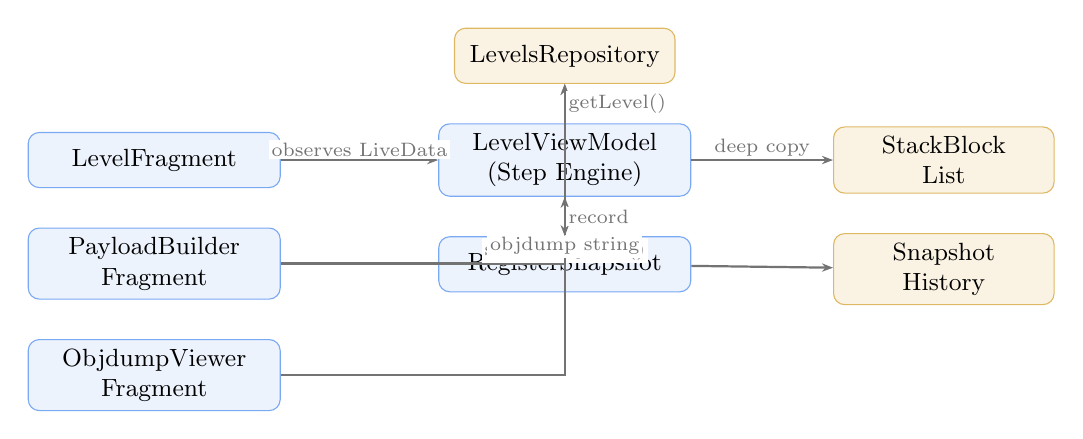
\begin{tikzpicture}[
    node distance=0.6cm and 1.8cm,
    box/.style={rectangle, rounded corners=4pt, draw=svblue!60,
                fill=svblue!8, minimum width=3.2cm,
                minimum height=0.7cm, font=\small, align=center},
    db/.style={rectangle, rounded corners=4pt, draw=svamber!70,
               fill=svamber!12, minimum width=2.8cm,
               minimum height=0.7cm, font=\small, align=center},
    arr/.style={-{Stealth[length=4pt]}, thick, black!55},
    lbl/.style={font=\scriptsize, fill=white, inner sep=1pt}
]
\node[box] (frag)   {LevelFragment};
\node[box, below=0.5cm of frag]  (pb)    {PayloadBuilder\\Fragment};
\node[box, below=0.5cm of pb]    (od)    {ObjdumpViewer\\Fragment};
\node[box, right=2cm of frag]    (vm)    {LevelViewModel\\(Step Engine)};
\node[db,  above=0.5cm of vm]    (repo)  {LevelsRepository};
\node[db,  right=1.8cm of vm]    (stack) {StackBlock\\List};
\node[db,  below=0.5cm of stack] (snaps) {Snapshot\\History};
\node[box, below=0.5cm of vm]    (snap)  {RegisterSnapshot};

\draw[arr] (frag) -- node[lbl,above]{\scriptsize observes LiveData} (vm);
\draw[arr] (pb)   -| node[lbl,pos=0.7,below]{\scriptsize submitPayload()} (vm);
\draw[arr] (od)   -| node[lbl,pos=0.7,above]{\scriptsize objdump string}  (repo);
\draw[arr] (vm)   -- node[lbl,above]{\scriptsize deep copy} (stack);
\draw[arr] (vm)   -- node[lbl,right]{\scriptsize getLevel()} (repo);
\draw[arr] (vm)   -- node[lbl,right]{\scriptsize record} (snap);
\draw[arr] (snap) -- (snaps);
\end{tikzpicture}
\caption{High-level architecture of \SV{}: presentation layer (left) $\to$
ViewModel step engine (centre) $\to$ data layer (right).}
\label{fig:arch}
\end{figure}

\subsection{Data Schema}

Each level is an immutable \texttt{Level} object with the fields shown in
Table~\ref{tab:schema}. Stack state is a \texttt{List<StackBlock>}, where each
block carries an address, label, value, size, and type constant
(\texttt{NEUTRAL}, \texttt{FILLED}, \texttt{SAFE}, \texttt{WARN}, \texttt{DANGER},
\texttt{JUNK}, \texttt{TARGET}).

\begin{table}[H]
\centering
\caption{Key fields of the \texttt{Level} data class}
\label{tab:schema}
\renewcommand{\arraystretch}{1.25}
\begin{tabular}{p{3cm} p{2.2cm} p{7cm}}
\toprule
\textbf{Field} & \textbf{Type} & \textbf{Description} \\
\midrule
\texttt{id}            & String           & \texttt{"1"}, \texttt{"2a"}, \texttt{"2b"}, \ldots \\
\texttt{goal}          & String           & Win token: \texttt{CRASH}, \texttt{LEAK}, \texttt{CFH} \\
\texttt{code}          & List<CodeLine>   & Source lines, each optionally carrying disassembly \\
\texttt{initialStack}  & List<StackBlock> & Immutable initial state; deep-copied on reset \\
\texttt{defensePatch}  & DefensePatch     & Before/after strings for the ``Apply Patch'' feature \\
\texttt{objdump}       & String           & Raw \texttt{objdump -d} output (nullable; used in L2B) \\
\bottomrule
\end{tabular}
\end{table}

\subsection{Development Methodology}

\SV{} is developed using an \textbf{Agile} approach with feature-focused sprints.

\begin{enumerate}[leftmargin=1.5em, itemsep=4pt]
    \item \textbf{Curriculum and Requirement Design.} Analysed existing resources
    (textbooks, CTF archives, web platforms) to map content gaps and define a
    seven-level progressive curriculum where each level introduces exactly one new
    exploitation concept.

    \item \textbf{Architecture and Data Model.} Established the MVVM layer
    structure using Android Architecture Components (LiveData, ViewModel). The
    \texttt{Level/StackBlock/RegisterSnapshot} schema was designed to support both
    the main execution engine and the payload builder wizard without duplication.

    \item \textbf{Iterative Implementation.} All logic is written in Java (API~26+).
    Deep-copy semantics for stack state ensure correct, aliasing-free snapshot
    restoration. The \texttt{StackCanvasView} uses \texttt{lerp()}-based
    interpolation for fluid ESP/EBP pointer animation.

    \item \textbf{Testing.} Each level's step engine is validated against fixed
    expected stack states. The payload builder wizard is validated against the correct
    exploit parameters (junk blocks 3--7, target block 2, address \texttt{0x400476}).
\end{enumerate}

% ══════════════════════════════════════════════════════════════════════════════
\section{Implementation Details}

\subsection{StackCanvasView --- Animated Memory Renderer}

\texttt{StackCanvasView} overrides \texttt{onDraw(Canvas)} to render the stack as
colour-coded labelled rectangles. Blocks are drawn top-to-bottom in descending
address order. A wave-animated \texttt{Path} over the buffer blocks
($6 \cdot \sin(\texttt{time} + i \cdot 0.3)$ wave displacement per frame) simulates
fluid overflow. In selection mode, block colours override to: junk range (red),
first tap (amber), confirmed target (accent blue). Invalid taps trigger a
\texttt{ValueAnimator} spring-shake (300\,ms). \texttt{onMeasure()} guarantees
$\geq$60\,dp per block, ensuring scrolling rather than clipping for large stacks.

\subsection{Level 2B --- Control-Flow Hijack}

Level~2B uses a \texttt{gets()}-vulnerable C program with \texttt{win()} at
\texttt{0x400476}. The stack is eight blocks (main frame, vuln return addr, saved
RBP, four buf blocks). The step engine fires \texttt{getsReached = true} at step~3,
which triggers a dialog in \texttt{LevelFragment} offering two paths:

\begin{itemize}[leftmargin=1.5em, itemsep=3pt]
    \item \textbf{Normal input} --- text field fills buf blocks normally; overflow
    into adjacent blocks marks them \texttt{TYPE\_DANGER}.
    \item \textbf{Generate payload} --- launches \texttt{PayloadBuilderFragment},
    a full-screen three-step wizard:
    \begin{enumerate}[leftmargin=1em]
        \item \textit{Junk range}: tap first block, tap last block on the live
        stack canvas (amber $\to$ red highlight).
        \item \textit{Address}: tap the block immediately above the junk range;
        invalid taps shake. Address input dialog shows live little-endian byte
        preview (\texttt{0x400476} $\to$ \texttt{76 04 40 00 00 00 00 00}).
        \item \textit{Preview and Exploit}: payload shown as annotated
        \texttt{\textbackslash x} bytes; ``Exploit'' calls
        \texttt{viewModel.submitPayload()} and advances the step engine to the
        return-address hijack branch.
    \end{enumerate}
\end{itemize}

On step~6 the ViewModel checks: if the target block holds \texttt{0x400476},
the win toast fires and the console prints the flag; otherwise a SIGSEGV state
is shown with a hint.

\subsection{ObjdumpViewerFragment and Time-Travel Debugging}

The \texttt{ObjdumpViewerFragment} renders the embedded \texttt{objdump} string in
a monospace \texttt{RecyclerView} with three colour tiers: symbol labels (accent
blue), section headers (green), instruction lines (light grey). Long-pressing a line
copies its leading address token to the system clipboard via
\texttt{ClipboardManager}.

The timeline stores a \texttt{List<RegisterSnapshot>} in LiveData. Tapping a
snapshot calls \texttt{restoreSnapshot()}, which writes all fields back to their
respective LiveData simultaneously. History is truncated only on the next user
action, implementing non-destructive rewind.

% ── References ───────────────────────────────────────────────────────────────
\newpage
\begin{thebibliography}{8}

\bibitem{guo2013}
Guo, P.~J. (2013). Online Python Tutor: Embeddable web-based program
visualization for CS education. \textit{Proc.\ SIGCSE '13}, pp.~579--584. ACM.

\bibitem{hundhausen2002}
Hundhausen, C.~D., Douglas, S.~A., \& Stasko, J.~T. (2002). A meta-study of
algorithm visualization effectiveness. \textit{J.\ Visual Languages \& Computing},
13(3), 259--290.

\bibitem{chapmanburket2016}
Chapman, P., \& Burket, J. (2016). CTF: State-of-the-art and the way forward.
\textit{Proc.\ USENIX ASE '16}. USENIX Association.

\bibitem{rescorla2018}
Rescorla, E. (2018). The Transport Layer Security (TLS) Protocol Version~1.3.
\textit{RFC 8446}, IETF.

\bibitem{kahn1996}
Kahn, D. (1996). \textit{The Codebreakers} (rev.\ ed.). Scribner.

\bibitem{erickson2008}
Erickson, J. (2008). \textit{Hacking: The Art of Exploitation} (2nd ed.).
No Starch Press.

\bibitem{shacham2007}
Shacham, H. (2007). The geometry of innocent flesh on the bone. \textit{Proc.\
CCS '07}, pp.~552--561. ACM.

\bibitem{litsurvey2026}
Bhatt, M., Eqbal, N., Verma, P., \& Chaudhary, S. (2026). SecViz Literature
Survey. Internal report, MIT MAHE, Manipal.

\end{thebibliography}

\end{document}
